% !TeX spellcheck = pt_BR

%%%%%%%%%%%%%%%%%%%%%%%%%%%%%%%%%%%%%%%%%%%%%%%
% Modelo adaptado do template original de
% Ted Pavlic (http://www.tedpavlic.com)
% Todos os créditos a ele.
%
% Na versão atual, o que foi modificado
% do original:
% Ajusta a numeração das questões e
% passa para português.
% Além de separar as configurações
% em um arquivo .cls separado.
%
% Crédito ao Roberto por ter feito
% a maior parte do trabalho de passar
% para o português e fazer outros
% ajustes para a versão atual deste template.
%%%%%%%%%%%%%%%%%%%%%%%%%%%%%%%%%%%%%%%%%%%%%%%


%----------------------------------------------------------------------------------------
%	PACKAGES E OUTRAS CONFIGURAÇÕES
%----------------------------------------------------------------------------------------

\documentclass{homeworkclass}

\usepackage{animate}


\usepackage{myMacros}


\hmwkTitle{Lista\ de\ Exercícios \#5}
\hmwkDueDate{Segunda,\ 07\ de\ Julho,\ 2019}
\hmwkClass{Elementos de Processamento de 	Sinais}
\hmwkClassTime{Segundas e Quartas: 08:00--10:00}
\hmwkClassInstructor{Prof.\ Sergio Lima Netto}
\hmwkAuthorName{Vinicius Mesquita de Pinho}
\hmwkAuthorShortName{Vinicius Mesquita}

\begin{document}

\maketitle

%----------------------------------------------------------------------------------------
%	SUMÁRIO
%----------------------------------------------------------------------------------------

%\setcounter{tocdepth}{1} % Uncomment this line if you don't want subsections listed in the ToC

\clearpage
\newpage
%\tableofcontents
%\newpage

%----------------------------------------------------------------------------------------
%	QUESTÃO 1
%----------------------------------------------------------------------------------------

% To have just one problem per page, simply put a \clearpage after each problem



\begin{homeworkProblem}
	\paragraph{Exercício} Projetar um filtro adaptativo atráves do algoritmo LMS para a aplicação de identificação de sistemas.
	
	\paragraph{O algoritmo} No LMS, os coeficientes $\wbf(n)$ são atualizados através da seguinte equação:
	\begin{equation}
		\wbf(n+1) = \wbf(n) + 2\mu e(n)\xbf(n),
	\end{equation}
	onde $e(n) = d(n) - y(n)$, é o erro entre o sinal de referência e a saída do filtro adaptativo, e $\xbf(n)$ é o vetor formado pelo sinal de entrada. 
	
	A Figura~\ref{fig:sis} apresenta o diagrama de blocos do sistema a ser implementado. O objetivo é identificar os coeficientes de um sistema desconhecido através de um filtro adaptativo. Faremos simulações com diferentes cenários. 
	\begin{figure}[!ht]
		\centering
		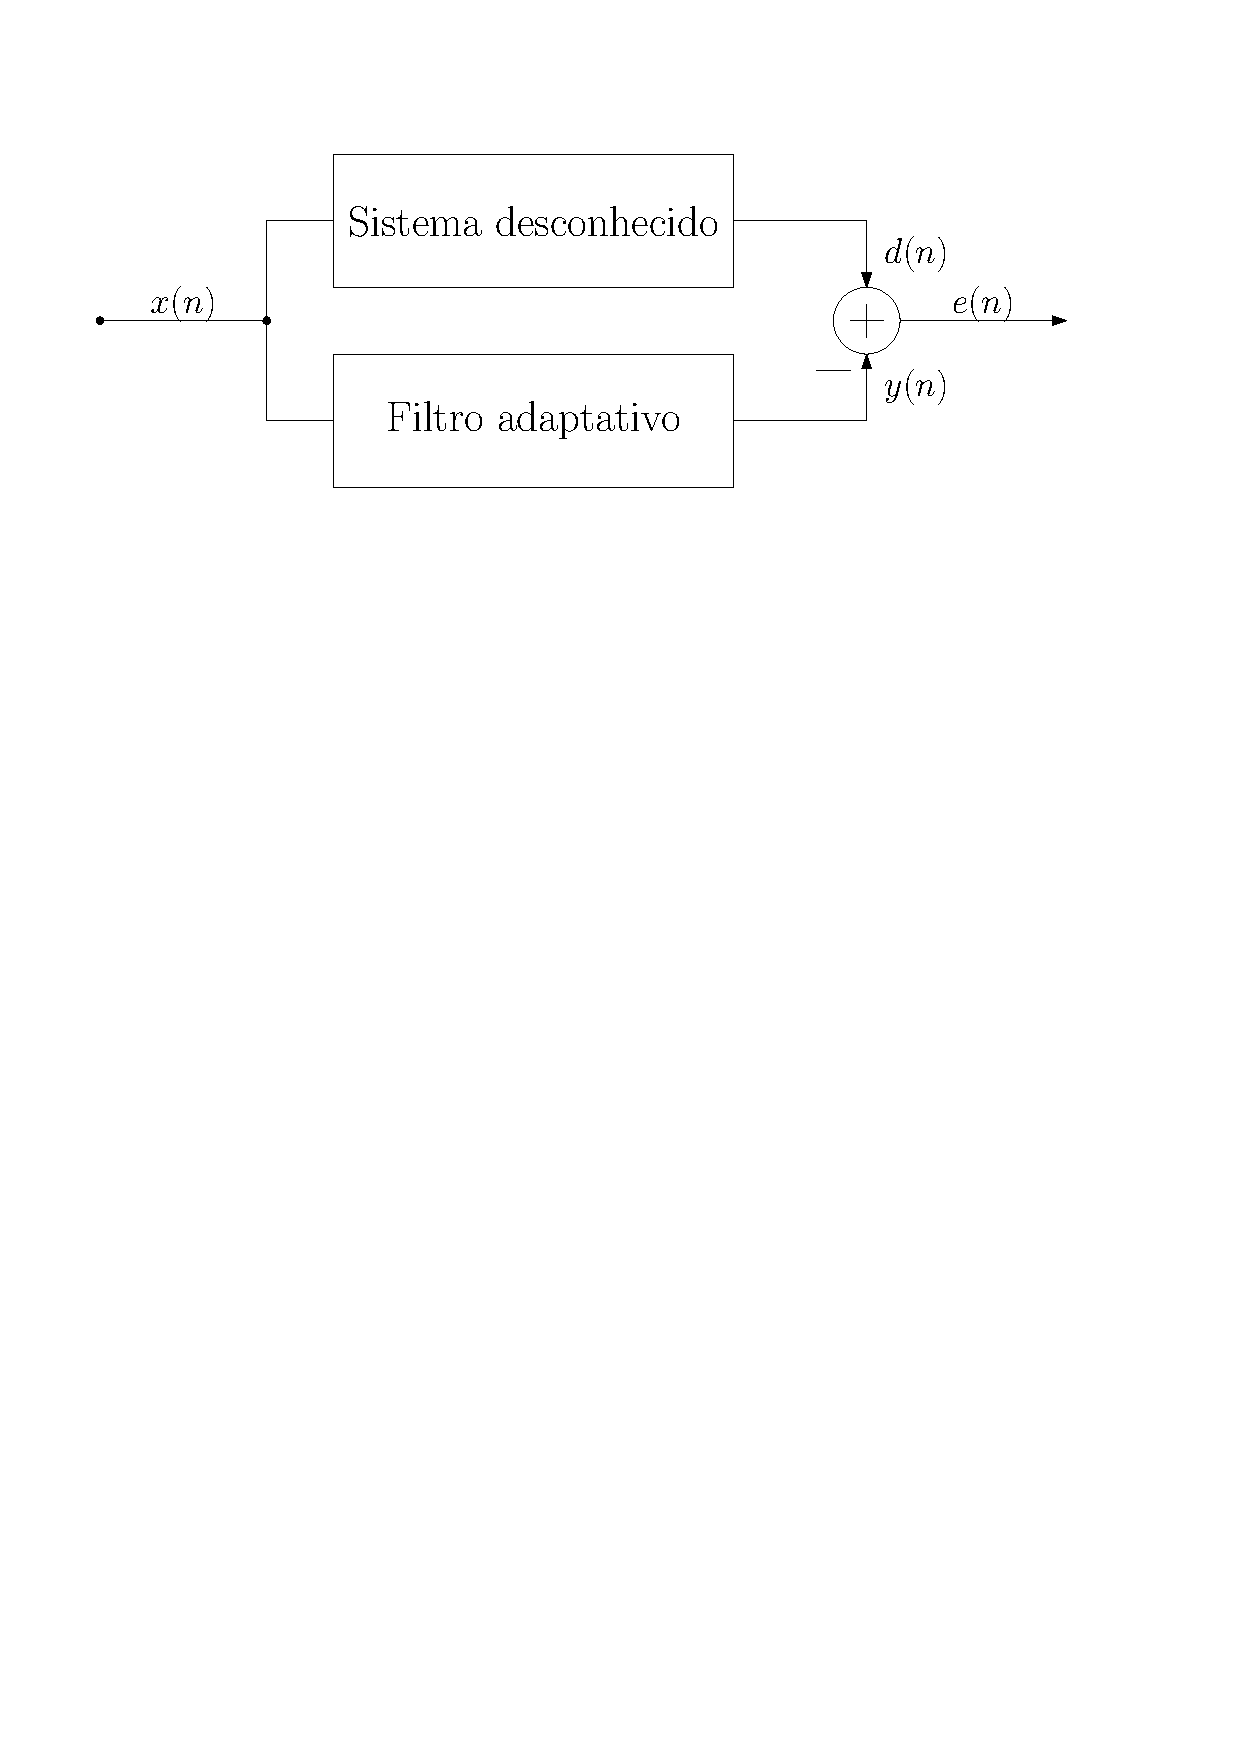
\includegraphics[width=0.6\linewidth]{figs/sistema}
		\caption{Sistema para identificação de sistema.}
		\label{fig:sis}
	\end{figure}
	
	\paragraph{Simulações}
	As simulações representarão três cenários diferentes, o caso em que o número de coeficientes do filtro adaptativo é o mesmo do sistema desconhecido, em outras palavras, acertamos a ordem do sistema desconhecido. Teremos também o caso em que o filtro adaptativo tem ordem superior ao do sistema desconhecido, e o caso contrário, em que o filtro adaptativo tem menos coeficientes que o sistema desconhecido. \\
	
	Para todas as simulações foram usados os seguintes parâmetros (a não ser quando explícita a mudança de um dos parâmetros padrões): \\
	
	\begin{tabular}[!ht]{|c|c|}
		\hline 
		\textbf{Parâmetro} & \textbf{Valor} \\ 
		\hline 
		Rodadas & 100 \\ 
		\hline 
		Iterações & 3000 \\ 
		\hline 
		$\mu$ & 0.025 \\ 
		\hline 
	\end{tabular}  \\ \\
	
	Para o primeiro caso, o sistema desconhecido e o filtro adaptativo tem a mesma ordem. No caso, os dois tem ordem 3. A Figura~\ref{fig:mselms} mostra o MSE (em dB) para diferentes valores de $\mu$. 
	
	\begin{figure}[!ht]
		\centering
		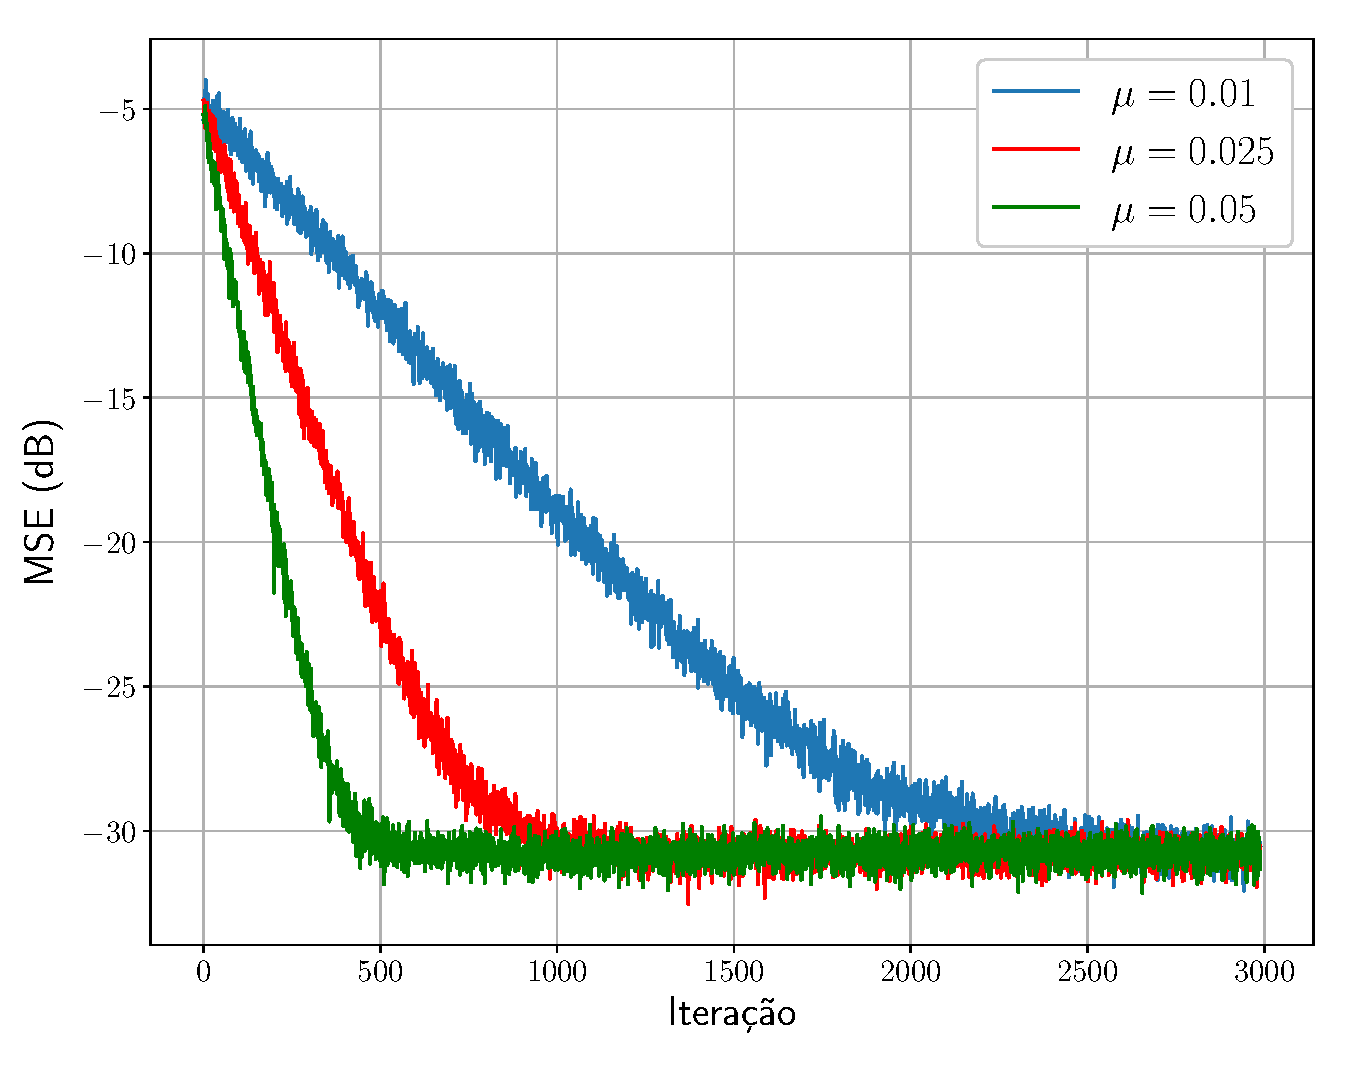
\includegraphics[width=0.6\linewidth]{figs/mse_lms}
		\caption{Curva de MSE (em dB) do algoritmo LMS.}
		\label{fig:mselms}
	\end{figure}
	
	\pagebreak
	
	No segundo caso o sistema desconhecido tem ordem superior ao do filtro adaptativo. Neste caso, se o sistema desconhecido tem $M$ coeficientes, o filtro adaptativo vai aprender os $N$ primeiros coeficientes do sistema desconhecido, onde $N$ ($M > N$) é o número de coeficientes do filtro adaptativo. A curva de MSE é muito semelhante a da Figura~\ref{fig:mselms}. 
	
	O terceiro caso é mais interessante que o segundo. Neste caso, o sistema desconhecido tem menos coeficientes do que o filtro adaptativo. Então, o filtro adaptativo vai ter os $N$ primeiros coeficientes iguais aos do sistema desconhecido (após a convergência), que tem $M$ $(N > M)$ coeficientes, o resto será tenderá a zero (serem nulos). 	Podemos ver a dinâmica dos coeficientes do filtroa adaptativo na Figura~\ref{fig:coef}. Para este exemplo, o filtro adaptativo tem $6$~coeficientes, enquanto o sistema desconhecido tem $4$~coeficientes. O que é interessante na Figura~\ref{fig:coef} é ver que 4 coeficientes convergem para os valores do sistema desconhecido, enquanto dois sobressalentes vão a zero.
	
	\begin{figure}[!ht]
	\centering
	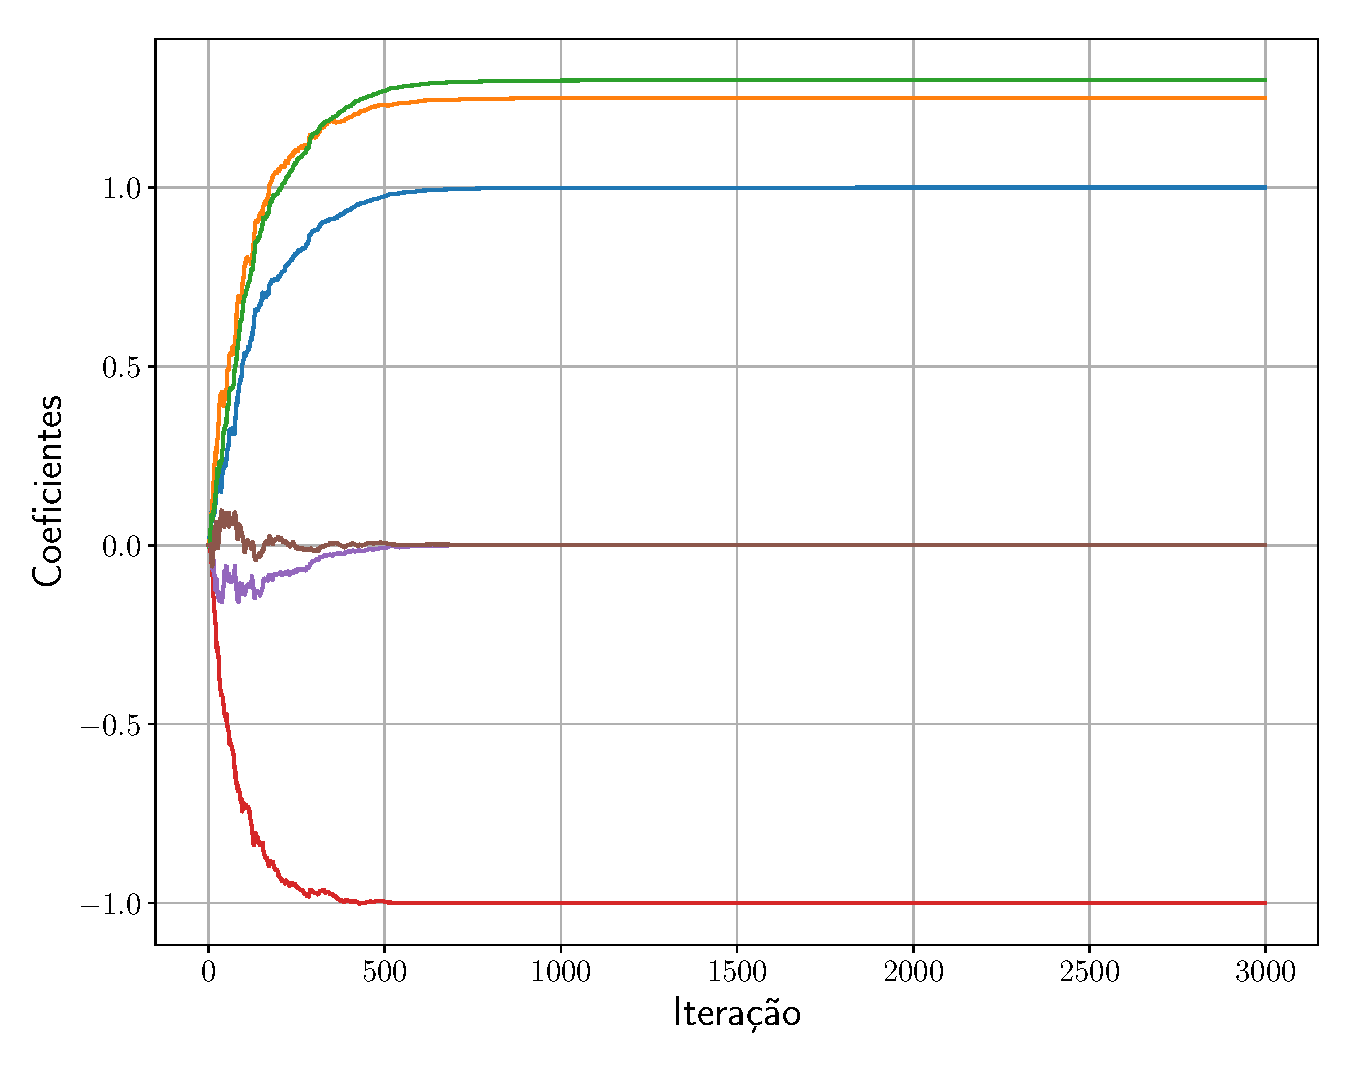
\includegraphics[width=0.5\linewidth]{figs/coeficientes}
	\caption{Variação dos coeficientes do filtro adaptativo.}
	\label{fig:coef}
	\end{figure}
	
	Podemos concluir então que é muito melhor ``errar para mais'' o número de coeficientes do seu filtro adaptativo.

\end{homeworkProblem}

\end{document}